%!TEX root=document.tex

\subsection{Pruning Optimizations}
\label{sec:custom_execution_engine_expts}
In Section \ref{sec:in_memory_execution_engine}, we developed a set of strategies that enable \SeeDB to eliminate aggregate views with low utility early on and identify top-$k$ aggregate views rapidly.
Through the next set of experiments, we evaluate 
the impact of these optimizations.
% Specifically, our evaluation studies the impact of
% (a) our pruning strategies, 
% (b) utility distributions for the dataset, and (c) parameters of our heuristics
% on latency and accuracy.
% Specifically, in addition to latency (i.e. time required for \SeeDB to produce recommendations),
% we evaluate whether the views chosen by \SeeDB actually have the highest utilities.

\stitle{Metrics:}
We evaluate performance of pruning optimizations along two dimensions, {\em latency}, as before, and
quality of results.
We measure the quality of results with two metrics: 
(1) {\em accuracy}: if $\{\mathcal{V}_T\}$
is the set of aggregate views with the highest utility and $\{\mathcal{V}_S\}$ is the set of 
aggregate views returned by
\SeeDB, the accuracy of \SeeDB is defined as $\frac{1}{\{|\mathcal{V}_T\}|} \times 
|\{\mathcal{V}_T\} \cap \{\mathcal{V}_S\}|$, i.e. the
fraction of true positives in the aggregate views returned by \SeeDB. 
(2) {\em utility distance}: since multiple
aggregate views can have similar utility values, we use utility distance as a measure of how {\it far} \SeeDB 
results are from the true top-$k$ aggregate views. 
We define utility distance as the difference between the average utility of $\{\mathcal{V}_T\}$ 
and the average utility of $\{\mathcal{V}_S\}$, i.e., $\frac{1}{n}(\sum_{i}U(\mathcal{V}_{T,i}) - 
\sum_{i}U(\mathcal{V}_{S,i}))$.

\noindent{\underline{Accuracy vs. Utility Distance.}} 
Since our pruning optimizations rely on utility estimates, the accuracy of pruning
depends on the differences between utilities of consecutive views.
Specifically, if $V_1 \ldots V_n$ is the list of aggregate views ordered by decreasing 
utility, then the accuracy of pruning is inversely proportional to 
the difference between the $k$-th highest utility and the $k+1$-st utility, 
i.e., $\Delta_k = U(V_k) - U(V_{k+1})$.
Views with large $\Delta_k$ values can be pruned accurately while whose with
small $\Delta_k$s can lead to lower absolute accuracy.
While this is true, notice that small $\Delta_k$s are, in fact, the result of views at 
the top-$k$ boundary having similar utility (and interesting-ness).
For instance, the utilities at the top-$5$ boundary for the DIAB dataset are 
$U(V_5)$ = 0.257, $U(V_6)$ = 0.254, and $U(V_7)$ = 0.252.
The small $\Delta_k$s lead to lower accuracy for $k$ = 5, but the 
very similar utility values indicate that $V_6$ and $V_7$ are (almost) equally interesting.
Therefore, even if $V_6$ or $V_7$ are incorrectly chosen to be in the top-$k$, 
the quality of results is essentially as high as when $V_5$ would have been chosen.
Our {\em utility distance} metric correctly captures this overall quality of results.
Utility distance indicates that, in the worst case, even when both $V_6$ or $V_7$ are 
incorrectly chosen, the overall utility of the top-$5$ differs only by 0.013 (~5\% error) 
units compared to the true top-$5$.
As a result, we jointly consider accuracy as well as utility distance when evaluating 
result quality.

% Therefore, when small $\Delta_k$ leads to lower accuracy, the same $\Delta_k$ guarantees that 
% the underlying small difference between utilities ensures that the views returned are {\it 
% just as interesting} as the true top-$k$.
% We refer to this as the {\it paradox of pruning}.

% Views with utilities that are spread apart can be pruned accurately while
% those with similar utilities can lead to pruning inaccuracies.
% The difference between utility values is particularly relevant at the top-$k$
% boundary.
 % to prune aggregate views, 
 % the accuracy of pruning depends on how accurately
 % our estimates can capture the relative order of utilities.
 % Aggregate views with utilities that are spread apart can be pruned accurately while
 % those with similar utilities can lead to pruning inaccuracies.
 % The difference between utility values is particularly relevant at the top-$k$
 % boundary.
 % Reusing notation from the MAB technique, if $V_1 \ldots V_n$ is the list of aggregate views 
 % ordered by decreasing utility, then the accuracy of pruning is inversely proportional to 
 % the difference between the $k$-th highest utility and the $k+1$-st utility, 
 % i.e., $\Delta_k = U(V_k) - U(V_{k+1})$.
 % If $\Delta_k$ is very small, the accuracy of our techniques is lower; however, the small 
 % $\Delta_k$ also implies that views around $k$ have almost equal utility.
 % For instance ...

\stitle{Techniques:}
In the following experiments, we evaluate four techniques for pruning low-utility views.
In addition to the two pruning strategies from Section~\ref{sec:pruning_opt}, 
namely the Hoeffding Confidence Intervals (CI) and the Multi-Armed Bandit (MAB),
we implement two baseline strategies.
First, the no pruning strategy processes the entire data and does not discard any views (NO\_PRU). 
It thus provides an upperbound on latency and accuracy, and lower bound on utility distance.
The other baseline strategy we evaluate is the random strategy (RANDOM) that returns a random 
set of $k$ aggregate views as the result.
This strategy gives a lowerbound on accuracy and upperbound on utility distance: for any 
technique to be useful, it must do significantly better than RANDOM.
Since absolute latencies of any pruning strategy depend closely on the exact DBMS execution techniques, 
in this section, we report relative improvements in latency, specifically, the percent improvement 
in latency with pruning compared to latency without pruning.
Absolute latency numbers for real datasets are discussed in Section \ref{sec:expt_summary}.

%we present latencies in this section 

\stitle{Datasets:}
Because pruning quality depends closely on the underlying data distribution, we evaluate
our pruning optimizations on the real-world datasets from Table \ref{tab:datasets}. 
In this section, we analyze the results for BANK and DIAB in detail; results for AIR and AIR10 are 
discussed in Section \ref{sec:expt_summary}. 
% \techreport{
% Specifically, we make use of the BANK and DIAB datasets listed in Table
% \ref{tab:datasets}. 
% Both datasets
% contain a mix of numerical and categorical attributes. 
% The diabetes dataset~\cite{diab} contains records of hospital visits by diabetes patients. Records include demographics,
% diagnoses, number of hospital days, and procedures performed. 
% The bank dataset~\cite{bank} contains records of customers who applied for a loan, including demographic information about 
% the customers, information about the bank's previous contact with the customer, and the ultimate loan decision.
% }





% For the custom execution engine, on the other hand, we are concerned with both, {\em latency} 
% as well as {\em accuracy}, i.e., whether \SeeDB actually returns the top-$k$ views or not.

% \techreport {
% \stitle{Result Highlights:}
% \begin{denselist}
% \item Our pruning strategies
% reduce \SeeDB latency from 20 seconds (without pruning in custom engine) to less than 2 seconds
% to return the first view, representing a {\em 10X reduction in latency}.

% \item Our latency improvements do not impact accuracy significantly;
% the accuracy of our results is $> 80\%$ with an almost zero utility distance.
% % the utility diof the returned views are close to the utilities
% % of the actual top-$k$ views.

% \item The distribution of (true) view utilities impacts accuracy of pruning strategies.
% Particularly, accuracy is inversely proportional to $\Delta_k$ the difference in
% utility between the $k$-th highest utility and the two neighboring utilities. 

% % \item Our technique of making a single pass through the data along with pruning reduces the overall
% % resource utilization of \SeeDB compared to the DBMS engine \mpv{quantify}.

% % \item Our  indicates that pruning significantly improves \SeeDB performance.
% % In addition, our requirement of only a single pass through the data reduces resource utilization.
% % Most importantly, 

% \item In all, the latency reduction of 10X (for top few views) -- 2X (overall) along with low
% utility distance enables \SeeDB to return high-quality recommendations {\bf at interactive time scales}.
% This makes the custom execution engine a better alternative to a DBMS-backed engine
% in terms of latency, accuracy as well as resource utilitzation (more in Section \ref{sec:comp_of_engines}).
% \end{denselist}
% }

% In addition to {\em latency}, we measure {\em accuracy},
% the number of true top-$k$ views present among the top-$k$ returned by the algorithm.
% In some cases, we will also measure {\em utility distance}, i.e., the 
% difference between the mean utility of the returned top-$k$ views
% and actual top-$k$ views.
% Unlike accuracy, which is 0-1, {\em utility distance}
% allows us to assess the benefit of strategies that return views with very high 
% (but not top) utilities.


% that have gone into We believe that comparing such
% systems offers little value:
% on one hand, our custom implementation lacks features such as logging or
% concurrency control that can slow down more complete systems; on the other hand,
% it also lacks optimizations for exploiting multiple cores, compression,
% vectorization, and other optimizations that scan-optimized column-stores employ.
% Rather, our goal is to highlight the relative performance benefits that can be
% obtained by performing pruning and shared scans.

\begin{figure}[h]
	\centering
	\begin{subfigure}{1\linewidth}
		\centering
		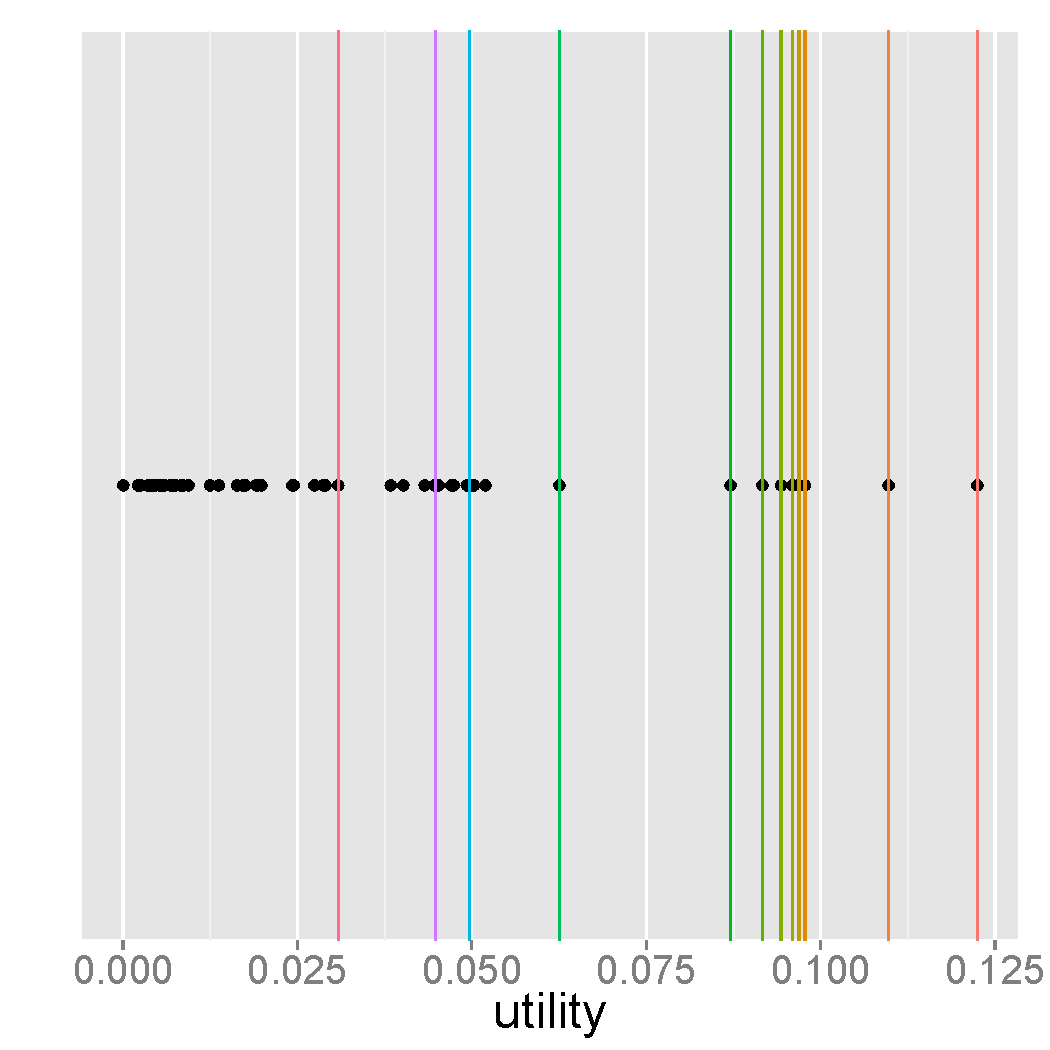
\includegraphics[width=6.5cm]
		{Images/bank_utility_distribution.pdf}
		\vspace{-5pt}
		\caption{Bank dataset: utility distribution}
		\label{fig:bank_utility_distribution}
	\end{subfigure}
	
	\begin{subfigure}{1\linewidth}
		\centering
		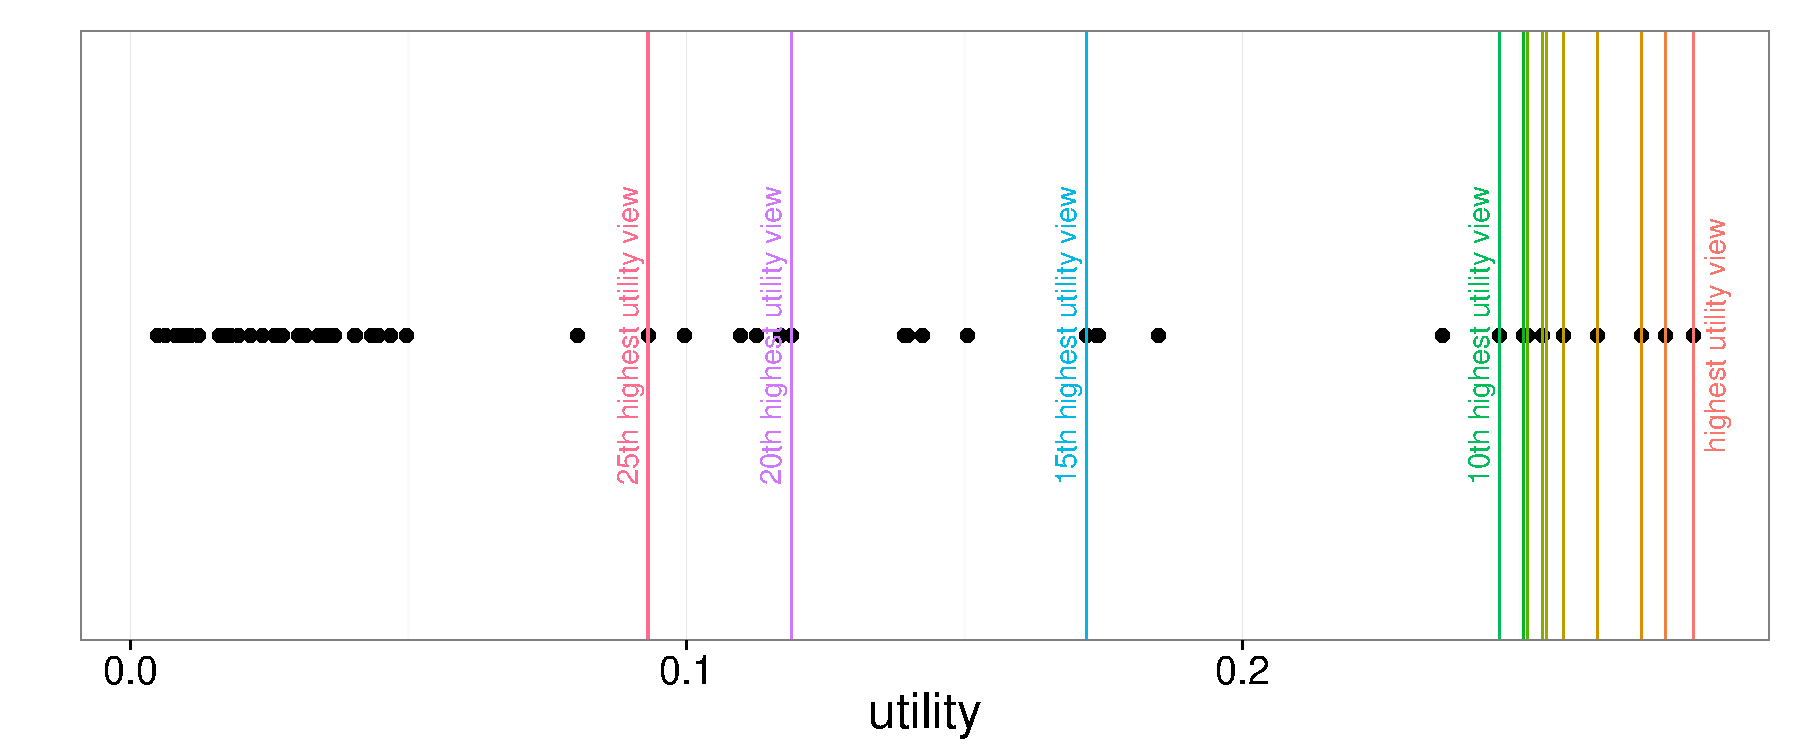
\includegraphics[width=6.5cm]
		{Images/diabetes_utility_distribution.pdf}
		\vspace{-5pt}
		\caption{Diabetes dataset: utility distribution}
		\label{fig:diabetes_utility_distribution}
	\end{subfigure}

\vspace{-10pt}
\label{fig:utility_distribution}
\caption{Distribution of Utilities}
\vspace{-15pt}
\end{figure}

In each of our experiments, we vary $k$ --- the number of visualizations to recommend --- between
1 and 25 (a realistic upper limit on the number of aggregates views displayed on a screen)
and measure the latency, accuracy, and utility distance for each of our
strategies. 
We pay special attentio to $k$ = 5 and 10 because empirically these $k$ values are used most commonly.
Since the accuracy and utility distance of our techniques are influenced by the
ordering of data, we repeat each experiment 20
times and randomize data between runs. We report average
metrics over 20 runs.
% We note upfront that our goal is not to directly compare the latency of our custom
% execution engine to that of the DBMS-backed execution
% engine; comparisons between a commercial DBMS-backed system and a proof-of-concept
% system are futile.
% Instead, our goal is to evaluate the performance improvements that can be
% obtained by pruning \techreport{and sharing table scans }in our proof-of-concept 
% implementation.\footnote{We note however that for our experimental datasets, 
% the proof-of-concept prototype provides performance comparable to the DBMS-backed
% system.} We start with an evaluation of the quality of results produced by our custom execution
% engine.

% For example, the DBMS-backed engines (especially the column store) benefits from 
% many man-years of optimizations, including optimizations for scan-intensive workloads, 
% vectorization, compression, the ability to exploit multiple cores and so on.  







% \begin{compactenum}[(a)]
%  \item Hoeffding Confidence Intervals (CI): we use Hoeffding-Serfling
%  confidence intervals with overall $\delta = 0.05$; 
%  % \item 95\% Confidence Intervals (95\_CI): this pruning strategy uses normal 95\% confidence intervals; and 
% \item Multi-armed Bandit (MAB): this pruning strategy uses the multi-armed bandit algorithm.
% \item No Pruning (NO\_PRU): this strategy returns the top-$k$ views with highest utility,
% with no intermediate pruning (to study the impact of pruning on latency);
% \item Random (RANDOM): this strategy returns randomly selected $k$ views (to study the impact of pruning on accuracy).
% \end{compactenum}

\begin{figure*}[t]
	\centering
	\begin{subfigure}{0.33\linewidth}
		\centering
		{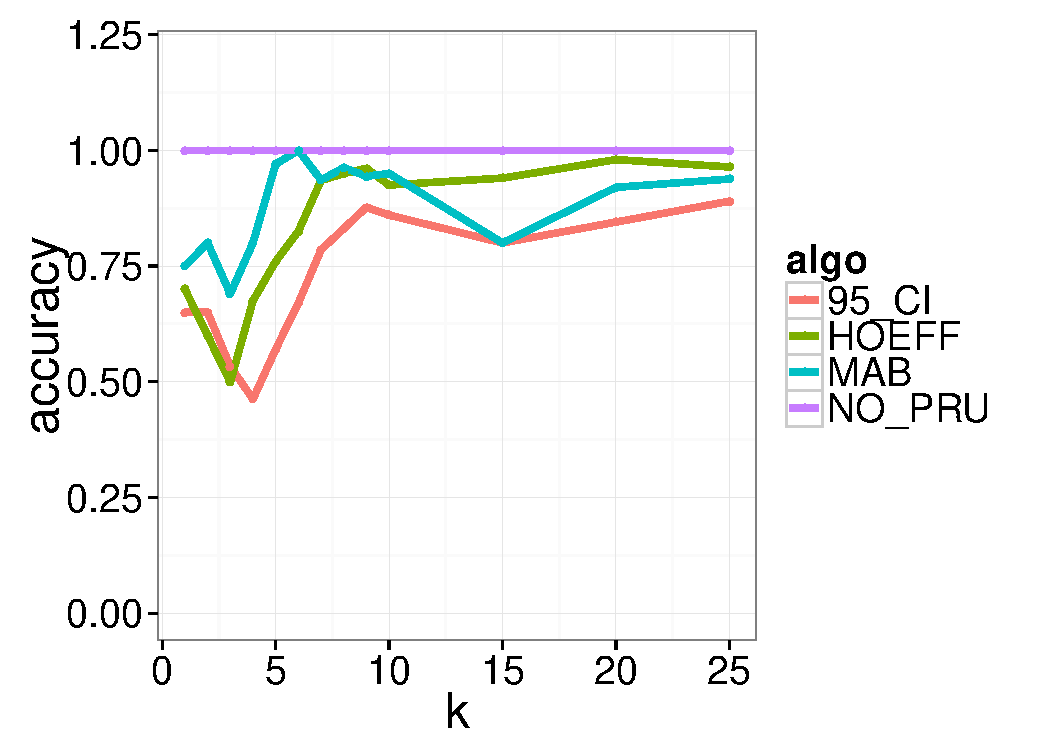
\includegraphics[width=6cm] {Images/in_memory_bank_accuracy.pdf}}
		\caption{Accuracy}
		\label{fig:bank_accuracy}
	\end{subfigure}
	\begin{subfigure}{0.33\linewidth}
		\centering
		{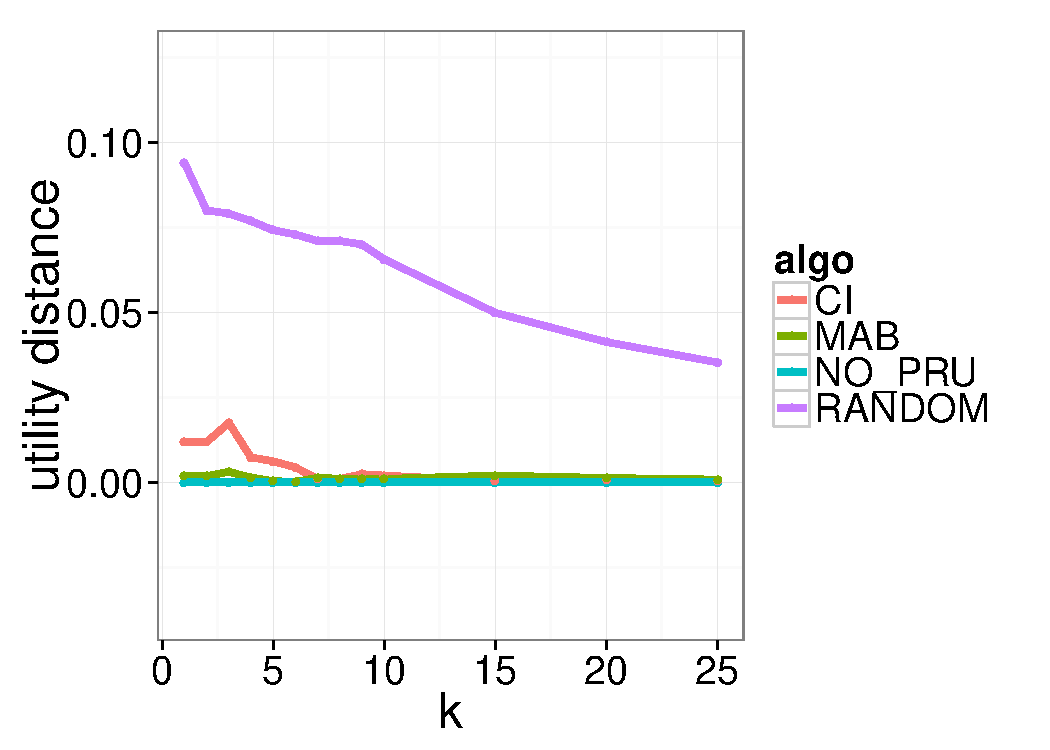
\includegraphics[width=6cm] {Images/in_memory_bank_utility_dist.pdf}}
		\caption{Utility Distance}
		\label{fig:bank_utility_dist}
	\end{subfigure}
	\begin{subfigure}{0.33\linewidth}
		\centering
		{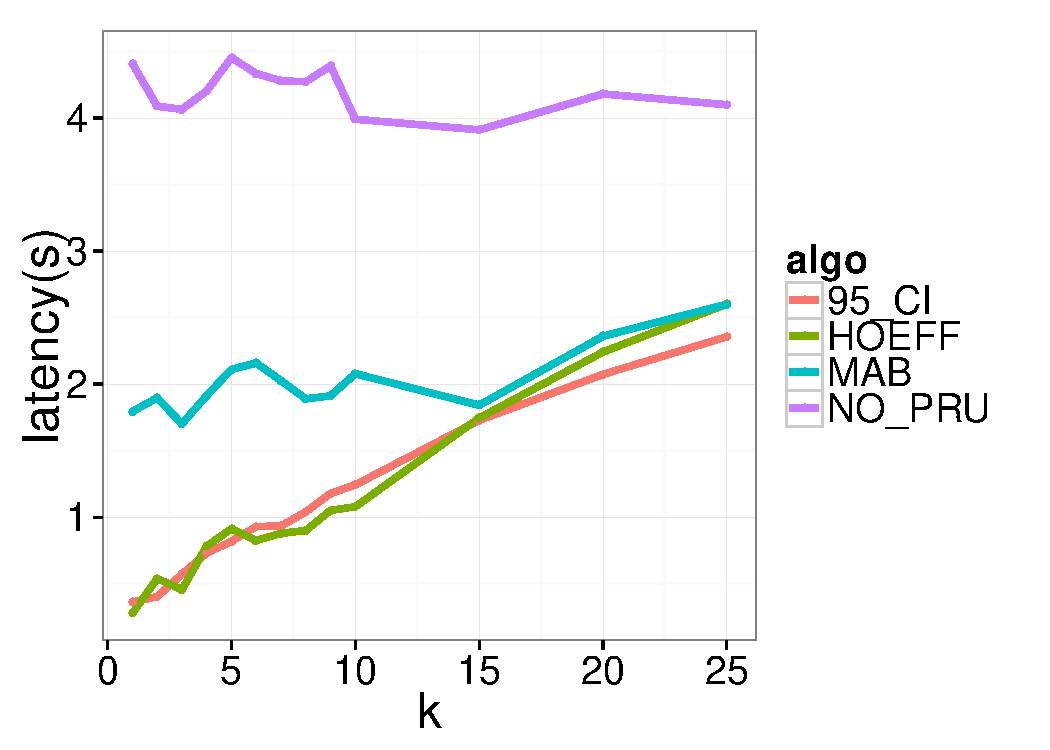
\includegraphics[width=6cm] {Images/in_memory_bank_latency.pdf}}
		\caption{Latency}
		\label{fig:bank_latency}
	\end{subfigure}
	\vspace{-10pt}
	\caption{Performance of strategies for Bank dataset}
	\label{fig:bank_perf}
	\vspace{-10pt}
\end{figure*}

\begin{figure*}[t]
	\centering
	\begin{subfigure}{0.33\linewidth}
		\centering
		{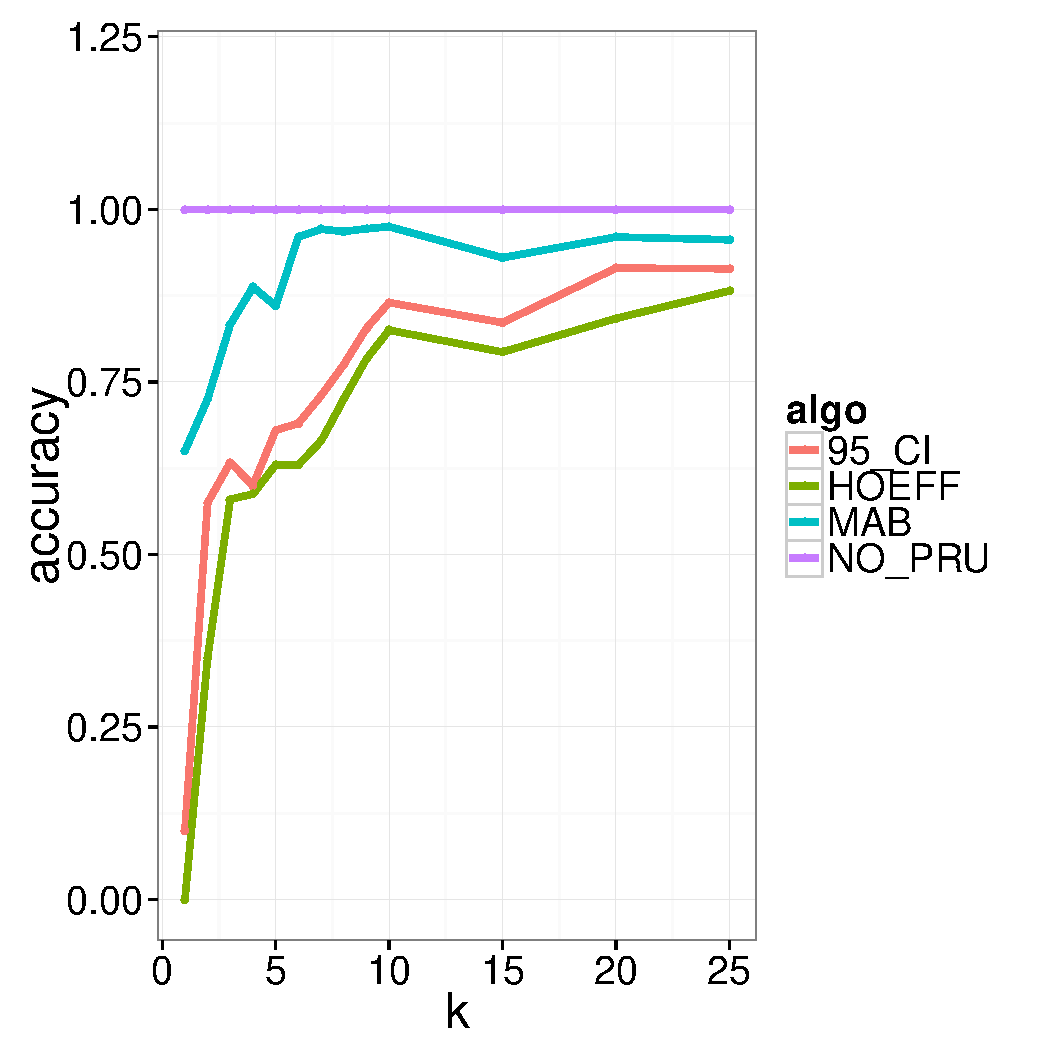
\includegraphics[width=6cm] {Images/in_memory_dia_accuracy.pdf}}
		\caption{Accuracy}
		\label{fig:dia_accuracy}
	\end{subfigure}
	\begin{subfigure}{0.33\linewidth}
		\centering
		{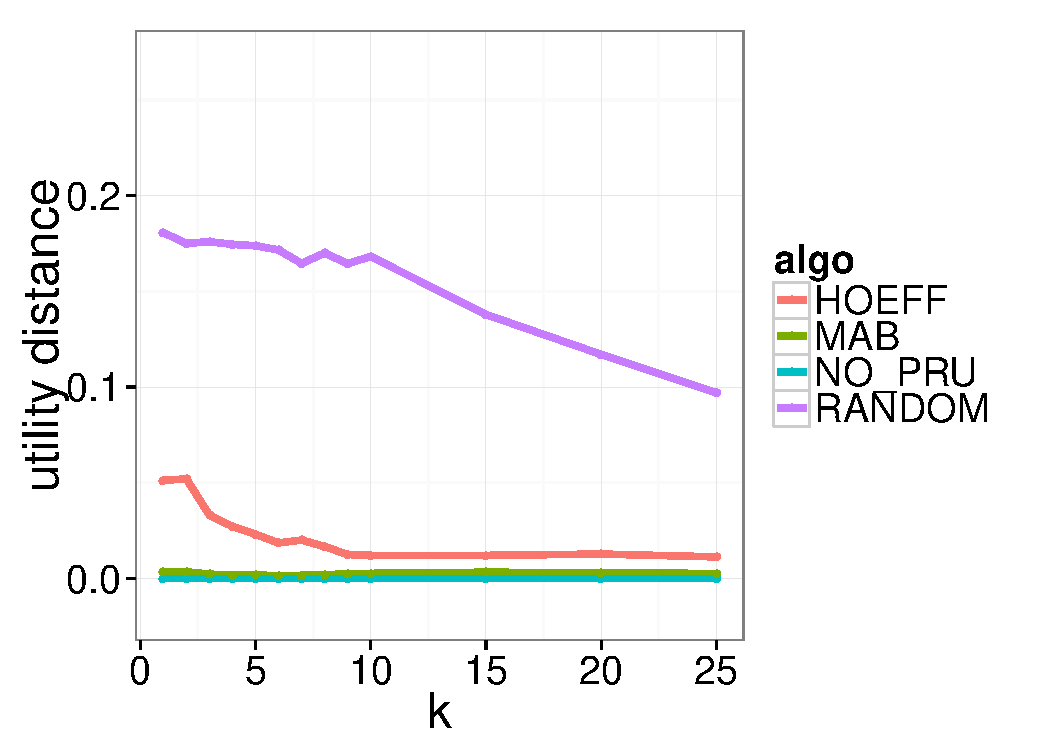
\includegraphics[width=6cm] {Images/in_memory_dia_utility_dist.pdf}}
		\caption{Utility Distance}
		\label{fig:dia_utility_dist}
	\end{subfigure}
	\begin{subfigure}{0.33\linewidth}
		\centering
		{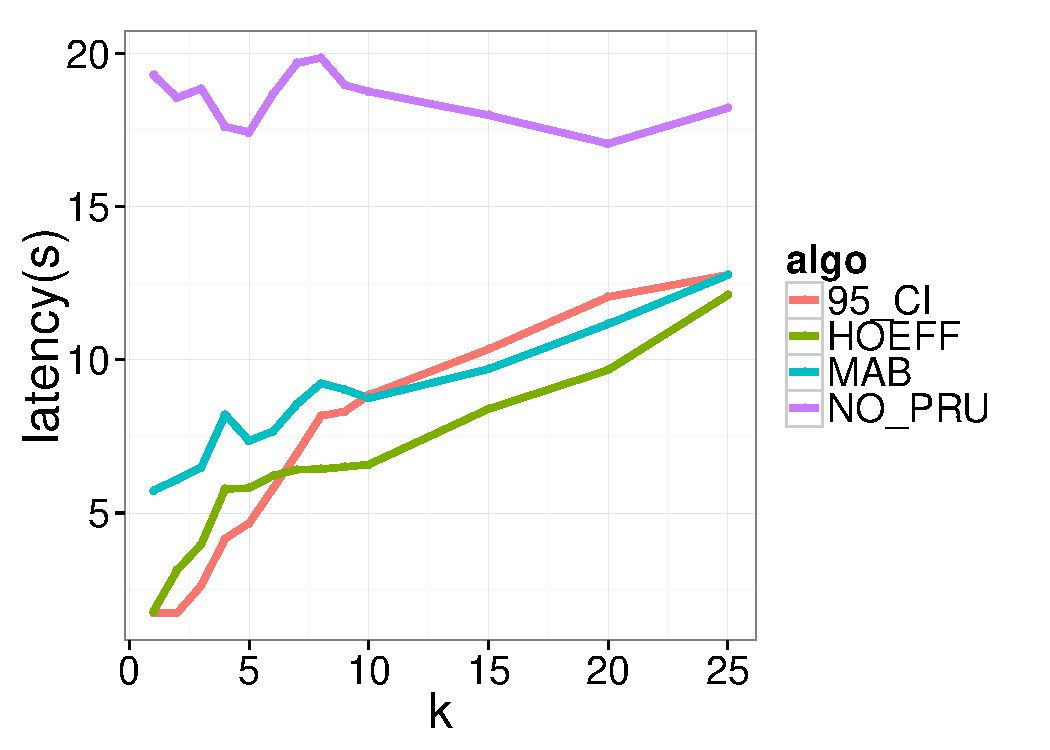
\includegraphics[width=6cm] {Images/in_memory_dia_latency.pdf}}
		\caption{Latency}
		\label{fig:diabetes_latency}
	\end{subfigure}
	\vspace{-10pt}
	\caption{Performance of strategies for Diabetes dataset}
	\label{fig:diabetes_perf}
	\vspace{-10pt}
\end{figure*}

 % \stitle{Utility Distributions and Quality of Results}:
 
 
 % Specifically, if a large number of views around the (true) top-$k$ boundary have similar utilities,
 % then our pruning strategies may choose views incorrectly at this boundary.
 % This results in lower accuracy.
 % On the other hand, since these views have utility similar to the true top-$k$ views, the
 % resulting utility distance is almost zero.
 %since utilities that are close together have very similar running
%estimates of utility and hence are difficult to tease apart and prune.
 % For each of the test datasets, we first review the utility distributions and then
 % analyze the performance of our pruning strategies given the utility distribution.

\stitle{Accuracy and Utility Distance:}
{\em \underline{Summary:} The MAB and CI strategy both produce results with 
accuracy $>$75\% and near-zero utility distance for a variety of $k$ values.
MAB does slightly better than CI when utlity values are closely spaced.
In general, smaller $\Delta_k$ values lead to lower accuracy, but this is offset by
lower utility distance that is a consequence of the smaller $\Delta_k$s. 
}

%  \em \underline{Summary:} The MAB strategy dominates the CI
% strategy when it comes to both accuracy and utility distance,
% with accuracy $>$75\%  for $k = 1$ and even larger for larger
% values of $k$, and a near-zero utility distance. 
% Smaller $\Delta_k$ values lead to lower accuracy, but this is offset by
% lower utility distance.
%  }

\noindent {\it \underline {BANK dataset}}:
The distribution of utilities for all aggregate views of the bank dataset is
shown in Figure~\ref{fig:bank_utility_distribution}. 
In this chart, vertical lines denote the cutoffs for utilities of the top-$k$ views
where $k$=\{1,\ldots,10,15,20,25\}.
The highest utility for this dataset corresponds to the {\it right-most} line
in this chart while the 25-th highest utility corresponds to the {\it left-most}
line. 
We observe that the highest and second highest utility are spread well apart 
from the rest ($\Delta_k$=0.0125). 
The top 3rd--9th utilities are similar ($\Delta_k$<0.002) while the 10th highest 
utility is well separated from neighboring utilities ($\Delta_{10}$=0.0125).
The remaining aggregate views once again have similar utilities ($\Delta_k$<0.001).
We see the effect of utility distribution in the performance of our pruning 
strategies.
Figure~\ref{fig:bank_accuracy} and Figure~\ref{fig:bank_utility_dist} respectively show
the {\em average} accuracy and utility distance of our strategies over 20 runs.
We find that MAB consistently produces 75\% or better accuracy for all values of $k$ and
CI produces 85\% or better accuracy for $k$$>$10.
For $k$=1 and 2, the accuracy is 75\% for both pruning strategies (due to large 
$\Delta_k$ values).
The corresponding utility distance is almost zero for MAB and about 0.015 for CI (note that these
are averages).
Between $k$=3\ldots9, the accuracy for all strategies suffers due to small $\Delta_k$s ($< 0.002$).
In spite of lower accuracies, note that utility distance is consistently small ($<$ 0.02).
After $k$=10, the performance of all our strategies improves once again and tends to 100\% accuracy and
0 utility distance.
We note that NO\_PRU necessarily has perfect performance, while RANDOM has extremely poor accuracy (<0.25) 
and utility distance ($>$5X that of CI and MAB). 

% As with accuracy, the utility distance tends to zero with large $k$s.
% All our strategies produce views with 0 or almost 0 utility distance for most $k$. 
% Thus, even if \SeeDB picks a few incorrect views, there is effectively no difference in the 
% utilities of these views and the true top-$k$ views.
% So even when a top-$k$ strategy picks a few incorrect views, the selected views
% have utility very close to the real top-$k$ views, i.e., are views are
% of high quality.
% This implies that even if our top-$k$ views are
% approximate, they are of high quality.
% Another way to analyze mistakes in the top-$k$ views is by examining if the an
% incorrectly returned view for the top-$k$ views also appears in the top-$2k$,
% top-$3k$ or top-$4k$.
% Figure \ref{} shows the results for the banking dataset.
% We see that XXX,



% \begin{figure}[h]
% \centering
% \begin{subfigure}{0.49\linewidth}
% \centering
% {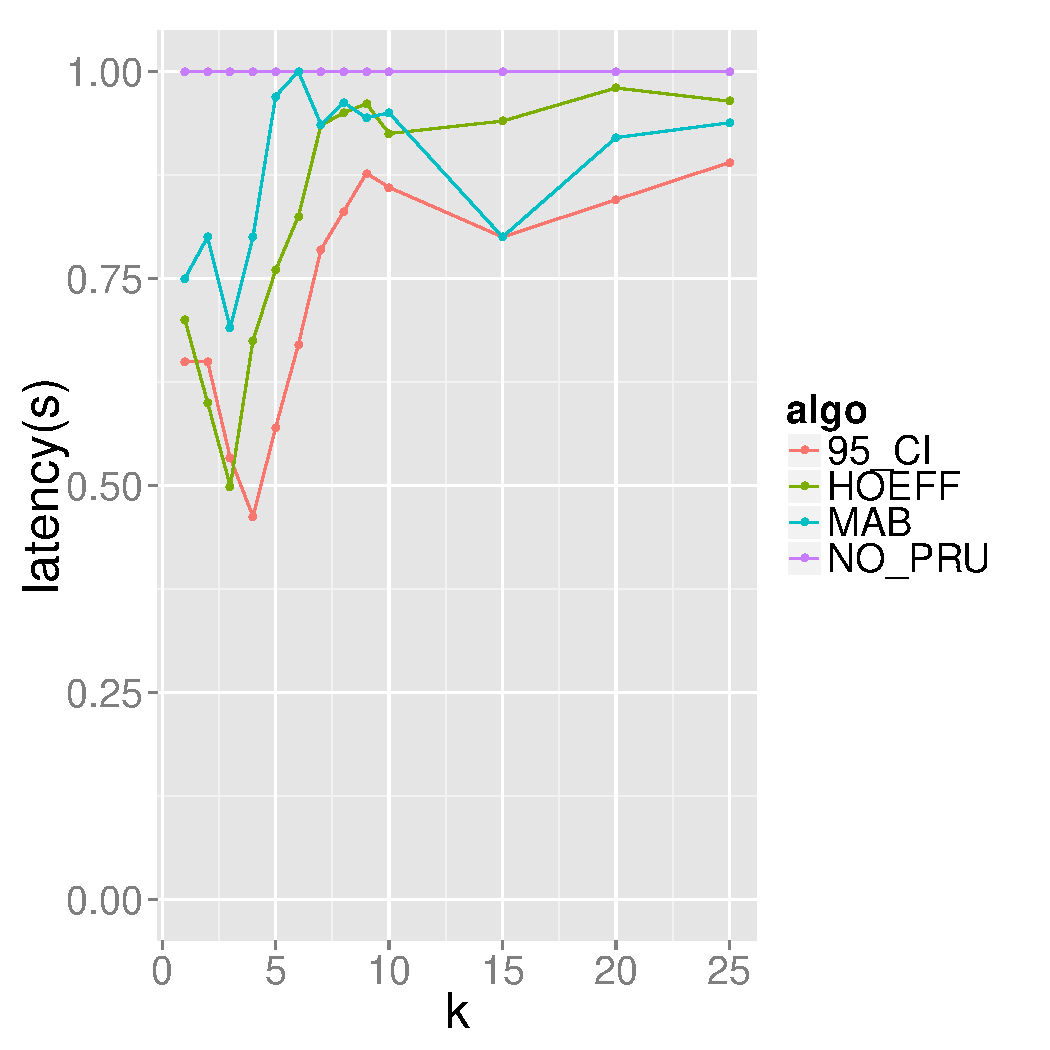
\includegraphics[width=4.2cm] {Images/bank_in_memory_accuracy.pdf}}
% \caption{Accuracy of strategy for bank dataset}
% \label{fig:bank_accuracy}
% \end{subfigure}
% \begin{subfigure}{0.49\linewidth}
% \centering
% {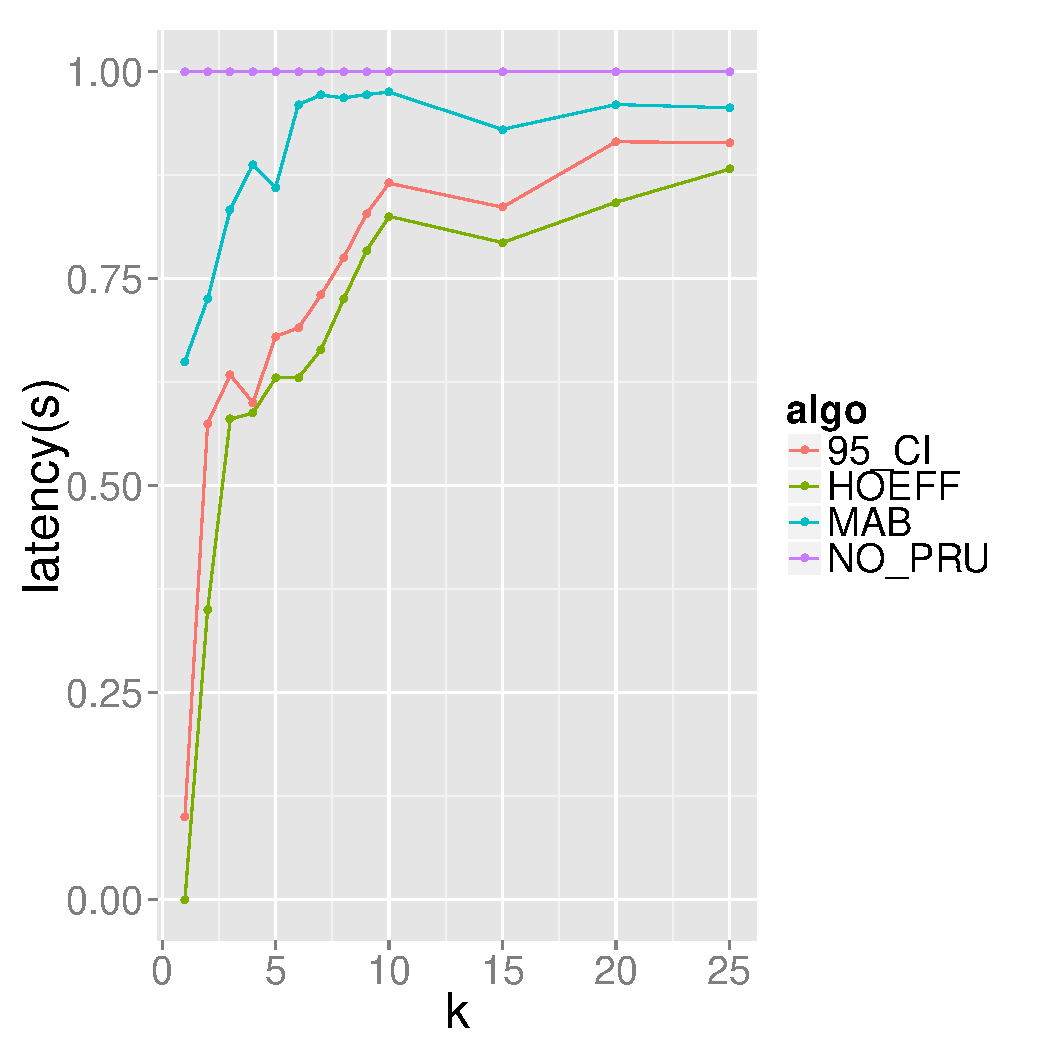
\includegraphics[width=4.2cm] {Images/dia_in_memory_accuracy.pdf}}
% \caption{Accuracy of strategies for diabetes dataset}
% \label{fig:dia_accuracy}
% \end{subfigure}
% \label{fig:accuracy}
% \caption{Accuracy of strategies}
% \end{figure}


% \begin{figure}[h]
% \centering
% \begin{subfigure}{0.49\linewidth}
% \centering
% {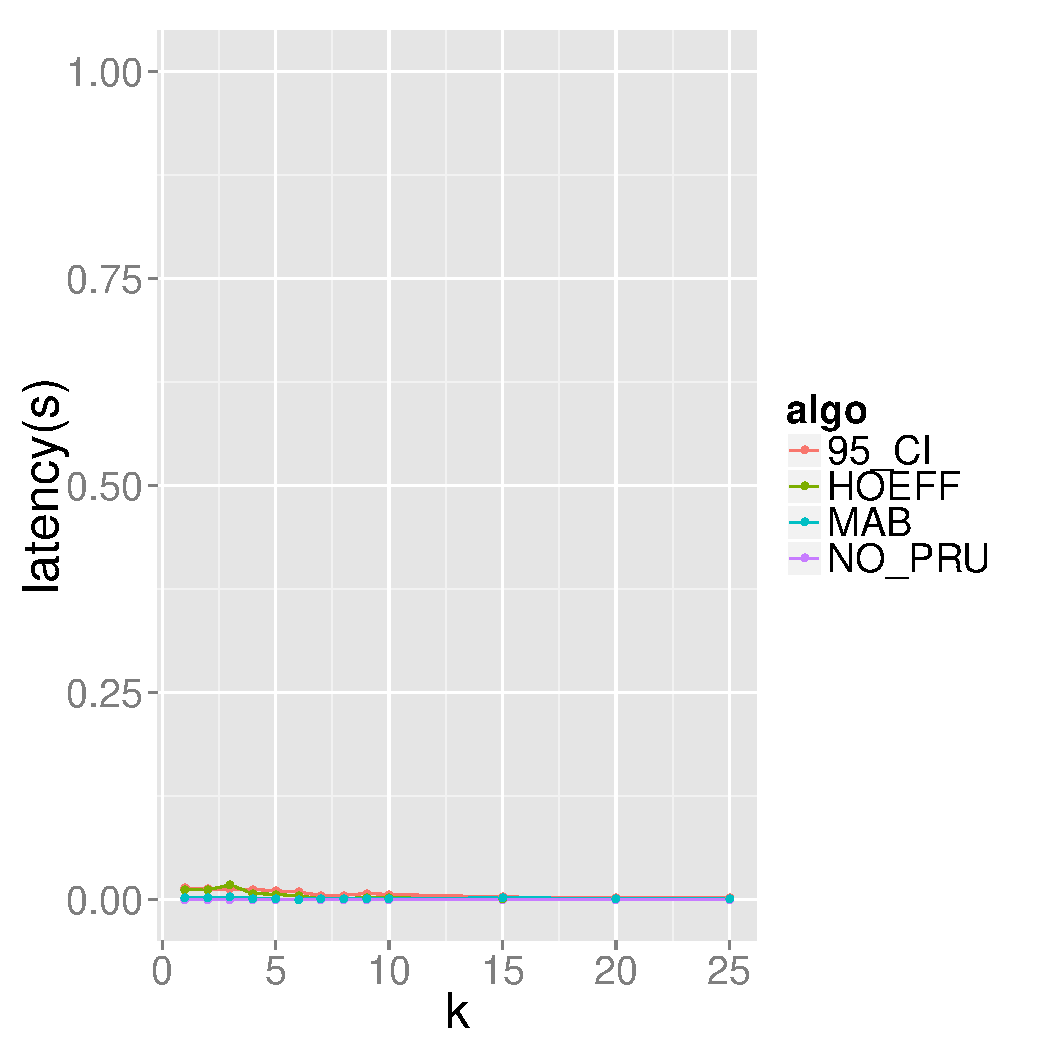
\includegraphics[width=4.2cm] {Images/bank_in_memory_utility_dist.pdf}}
% \caption{Utility Distance of strategy for bank dataset}
% \label{fig:bank_utility_dist}
% \end{subfigure}
% \begin{subfigure}{0.49\linewidth}
% \centering
% {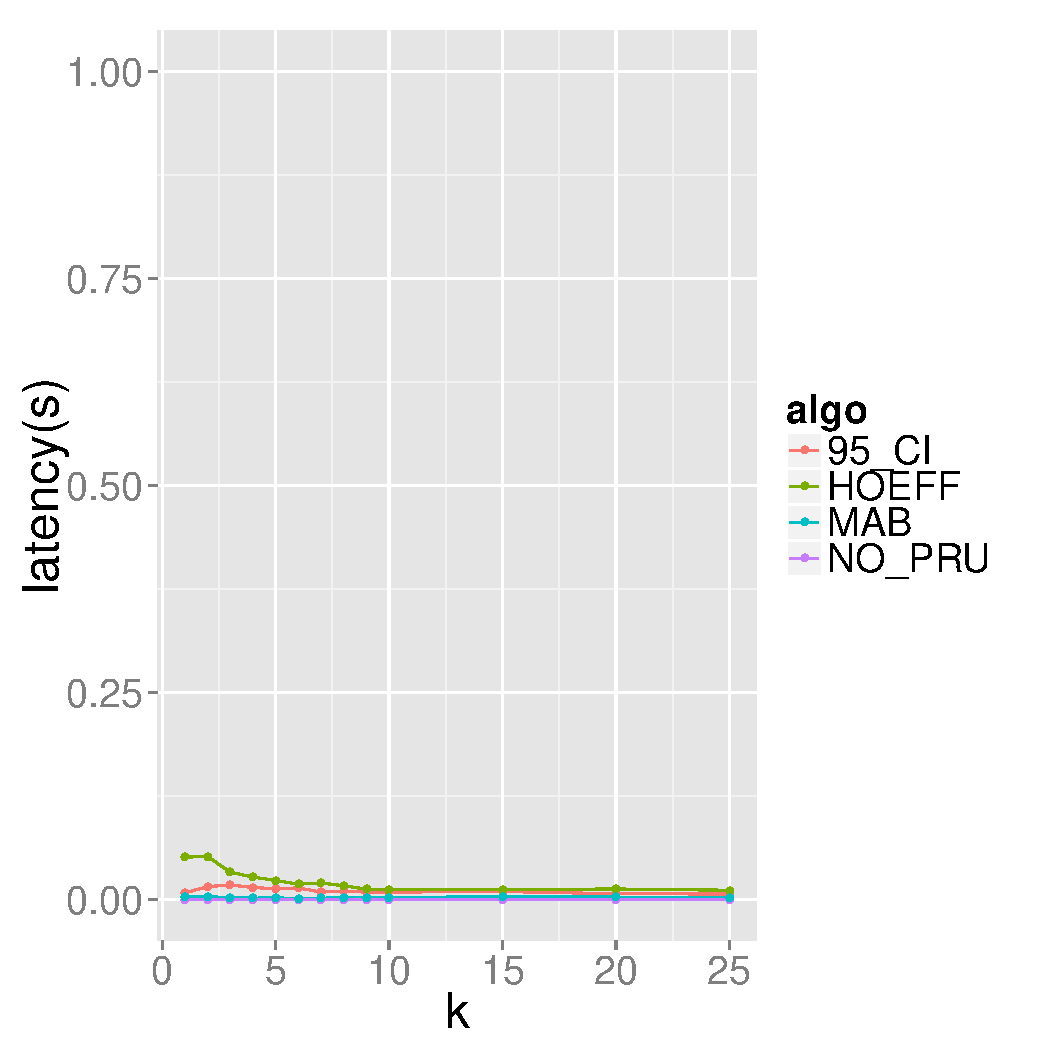
\includegraphics[width=4.2cm] {Images/dia_in_memory_utility_dist.pdf}}
% \caption{Utility Distance of strategies for diabetes dataset}
% \label{fig:dia_utility_dist}
% \end{subfigure}
% \label{fig:accuracy}
% \caption{Utility Distance for strategies}
% \end{figure}

% \begin{figure}[h]
% \centering
% {\includegraphics[trim = 0mm 50mm 0mm 50mm, clip, width=6cm]
% {Images/bank_utility_distribution.pdf}}
% \caption{Bank dataset: utility distribution}
% \label{fig:bank_utility_distribution}
% \end{figure}
% \begin{figure}[h]
% \centering
% {\includegraphics[trim = 0mm 50mm 0mm 50mm, clip, width=6cm]
% {Images/diabetes_utility_distribution.pdf}}
% \caption{Diabetes dataset: utility distribution}
% \label{fig:diabetes_utility_distribution}
% \end{figure}
 
\noindent {\it \underline{DIAB dataset:}} 
Next, we briefly review results for the diabetes dataset.
The distribution of true utilities for all aggregate views in this dataset are shown in
Figure~\ref{fig:diabetes_utility_distribution}.
We observe that utilities for the top 10 aggregate views are very closely clustered ($\Delta_k<$0.002) while
they are sparse for larger $k$s.
Therefore, we expect lower pruning accuracy for $k<10$ but high accuracy for
large $k$'s.
We see this behavior in Figure~\ref{fig:dia_accuracy} where the accuracy of
pruning is quite low ($<60\%$) for $k$=1 but improves consistently to 68\% (CI) 
and 86\% (MAB) for $k$=5 and is $>$80\% for $k$$\geq$10.
In the companion figure, Figure \ref{fig:dia_utility_dist}, we see that although
accuracy is relatively low $k$$<$5, utility distance is small (0.013 for CI, 0.002
for MAB) indicating that the results are high quality.
Both CI and MAB produce 40X smaller utility distances compared to RANDOM.

% We also observe an important property of our strategies: the accuracy of both
% of our pruning strategies, MAB and CI, is comparable; MAB appears to
% perform better for small number of $k$s but all three produce similar results
% for $k>10$. (NO\_PRU is guaranteed to have perfect accuracy).
% This suggests that since all strategies perform similarly on accuracy, we can
% choose the strategy with the minimum latency.\\

% 95\_CI does the best among all our strategies for the whole range of $k$ values.
% MAB and HOEFF produce similar accuracy values with MAB being slightly better
% than HOEFF.
% There are a few reasons why 95\_CI performs better: the MAB strategy is tied to
% either accepting or discarding a view at the end of each phase; therefore, even
% if MAB is not very confidence in the action of accepting or discarding, it must
% reduce one view in each phase. HOEFF on the other hand is less accurate because
% XXX.
% All our strategies however seem to have low accuracy for $k<10$. 

\stitle{Latency:}
{\em \underline{Summary:} Both pruning strategies provide a reduction in latency of 50\% or more
relative to NO\_PRU. For smaller $k$, reductions can be even higher, closer to 90\%; this can be
especially useful when we want to identify and quickly display the first one or two top views.}
Figures~\ref{fig:bank_latency} and \ref{fig:diabetes_latency} show the latency
of our strategies for the banking and diabetes dataset.
First off, we observe that the use of either of CI or MAB produces a 50\% reduction in latency
throughout.
In fact, for CI, we obtain almost a 90\% reduction in latency for small $k$. 
For $k$=5, MAB produces betwen 50 - 60\% reducation while CI produces a reduction of 60 - 80\%.
Early stopping, i.e. returning approximate results once the top-$k$ views have been identified, 
can produce even better latency reduction (results in Section \ref{??}).
As expected, as $k$ increases, latency also increases because we can prune fewer aggregate views.
% These reductions bring latency down from multiple tens of seconds to {\bf single digit latencies}, i.e.,
% \SeeDB can operate on interactive time scales.
% Since these latency numbers come from our prototype implementation, a well-tuned system could
% produce results in few seconds, i.e., {\it in interactive time scales}. 
% Clearly, we give up some accuracy when we obtain this reduction in latency, however, as demonstrated
% experimentally, our strategies consistently provide high utility views with low utility distance.op-$k$.
% This latency-accuracy tradeoff is particularly important in a real-time system where we want to quickly 
% provide recommendations for the analyst to browse.

\stitle{CI vs. MAB}.
In our evaluation, we compared two competing pruning strategies, CI and MAB. 
From Figures \ref{fig:bank_perf} and \ref{fig:diabetes_perf}, we observe that MAB, 
on average, has higher accuracy and lower utility distance compared to
CI, i.e., overall, it produces higher quality results.
However, we find that CI performs much better than MAB on latency.
Since CI can prune views more aggressively than MAB (MAB only discards one view at a time),
it can rapidly prune the space of views, but this comes at the cost of result quality.
Depending on the tradeoff between latency and quality of results, we can choose the best
pruning strategy from CI and MAB.

% \techreport{
% \stitle{Resource Utilization:}
% % \mpv{Not sure about this section. Someone needs to review}
% % We contrast the resource utilization of our custom execution engine to the DBMS-backed engine. 
% % Specifically:
% Compared to the resource utilization in the DBMS-backed engine, our custom engine requires much fewer resources.
% Specifically, since the custom engine makes a single pass through the data, the CPU utilization is expected to be lower compared to the repeated scans of the DBMS-backed engine.
% Another consequence of the single scan is that there is
% no thrashing introduced by multiple parallel scan queries.
% Lastly, there is no {\it query bloat} associated with
% the custom engine, saving overheads of per-query state such as iterators, buffers etc.
% }
% means that the custom engine is expected to
% have lower CPU as compared to the multiple scans of data resulting from the DBMS-backed engine (assuming that the
% additional state maintenance is not significant).

% Each \SeeDB query translates to only a single query in the custom execution engine.
% The DBMS-backed engine, in contrast, issues $~$ 50 queries for each \SeeDB query. 
% Consequently, additional resources must be wasted by the DBMS in keeping state for each query such as 
% iterators, buffers etc.

% \techreport{
% \subsection{Comparison of Execution Engines}
% \label{sec:comp_of_engines}

% The previous sections discussed the performance of the DBMS-backed and Custom execution engines of \SeeDB.
% We found that with a set of clever optimizations, we could reduce the latency of the DBMS-backed engine by
% 20X.
% However, the resulting latency of few tens of seconds was too large for interactive visualization.
% In addition, we found that the query bloat led to large memory footprint, repeated scans of data, and
% higher resource utilization.
% In contrast, the custom engine provided a means to perform a single scan of the data and identify top-$k$ views
% with high accuracy. \mpv{numbers?}
% Moreover, the custom engine produced latencies of a few seconds -- {\bf it enabled \SeeDB to respond at interactive
% time scales}.
% These performance results together indicate that the custom execution engine and its pruning strategies are a superior 
% alternative to a DBMS-backed execution engine.
% Since the goal of \SeeDB is to provide recommendations in real time, we can pay a small penalty in accuracy 
% and instead provide almost instantaneous results.

% Clearly, the ideal solution would be to integrate the custom execution engine functionality into a vanilla database.
% This would enable the DBMS to use existing structures to efficiently scan a dataset while maintaining and pruning
% views on the fly. 
% The SQL GROUPING SETS\footnote{} functionality, i.e. multiple independent group-bys in a single query is a first step in this direction.
% However, GROUPING SETS needs to be supplemented with much finer control and scalability to support \SeeDB-like  functionality.}

% In summary, the performance results of this section indicate that due to the lower latency, high accuracy,
% and overall lower resource utilization, the custom engine is a superior alternative to a DBMS-backed
% execution engine.
% It enables \SeeDB to make a single pass through the data, avoids unnecessary {\it query bloat} leading to
% lower resource utilization and lowers latency by upto 10X enabling \SeeDB to work in a real 
% interactive visualization system.

% so all of these strategies are promising alternatives to use 
% in a production system --- especially when we want to quickly identify and provide a few 
% views for the analyst to browse.
% If latency is paramount, then CI may be used,
% and if utility is paramount, then MAB may be used. \mpv {counter-intuitive}
% We observe that the latency of CI increases almost linearly
% with $k$. This trend arises because as $k$
% increases, we throw out fewer views and therefore perform more
% computation per record.
% This exact trend is not seen in MAB because MAB's view pruning is agnostic
% to the number of views that must be selected.

% \subsection{Combining Sharing \& Pruning}
% \label{sec:sharing_and_pruning}
% As discussed in the previous sections, sharing optimizations can provide performance gains upto 10X for COL and 40X for ROW while pruning optimizations can reduce latency by 2X -- 5X.
% In this section, we evaluate the performance gains that can be obtained by combining both types of optimizations. 
% In the ideal case, we expect the gains to be {\it multiplicative}, i.e., we would expect gains between 20X -- 200X.



% Figure \ref{fig:share_prune_col} shows the relative performance gains that can be obtained by applying various combinations of optimizations in the COL store. 
% As seen in figure, 

% The corresponding data for ROW stores was presented in Figure~\ref{fig:share_prune_row} above.
% We find that the combination of optimizations produce gains of upto 50X (COMB) -- 150X (COMB\_EARLY) for ROW, with pruning-based
% optimizations providing a 4X speedup over the sharing optimizations.


% We see similar results for ROW where pruning provides a similar 4X speedup.
% However, we make a few observations. First, pruning doesn't benefit small datasets (e.g. BANK, DIAB). In fact, due to the overhead of multiple phases (and the associated query costs), the combined optimization (COMB) does worse than SHARING alone. Since the SHARING latencies for small datasets are under a few seconds, we do not find the need to perform sharing.
% Second, as noted before, due to different data layout, COL stores have significantly lower latencies for the \SeeDB workload compared to ROW.
% However, the data layout for ROW benefits more from the sharing of scans and pruning since the cost of a table scan is much higher for ROW.
% T
% COL stores in general are a better fit for the \SeeDB workload.

% Compared to the performance of ROW stores in Figure \ref{}, we find that COL stores benefit less from optimizations.
% As before, this is because column stores can selectively load attributes that are relevant for the particular visualization. \mpv{verify}

% % We also find a few differences in the performance gains obtained by pruning in Section \ref{} () and those obtained by the combined optimizations ().

% The reasons for this difference are two-fold: (1) the simple pruning implementation described in Section \ref{} is based on shared scans and does not incur any overhead for each phase of the algorithm; in contrast, when we implement pruning in \SeeDB, each phase involves \SeeDB issuing a large number of queries to the DBMS and thus incuring overheads such as query dispatch, maintaining query state etc. (2) due to the specific implementations of ROW and COL stores, there is threshold on table size below which the time to scan tables is essentially the same.
% As a consequence of these two factors, we find that the combination of pruning and sharing degrades performance for small datasets (e.g. BANK, DIAB) due to phase overhead.
% The combination of optimizations is well suited to moderate and large datasets such as AIR and AIR10 and produces a CCC speedup.



% The next set of experiments vary the parameters for each strategy to study
% the accuracy vs. latency tradeoff.

% \begin{figure}[h]
% \centering
% \begin{subfigure}{0.49\linewidth}
% \centering
% {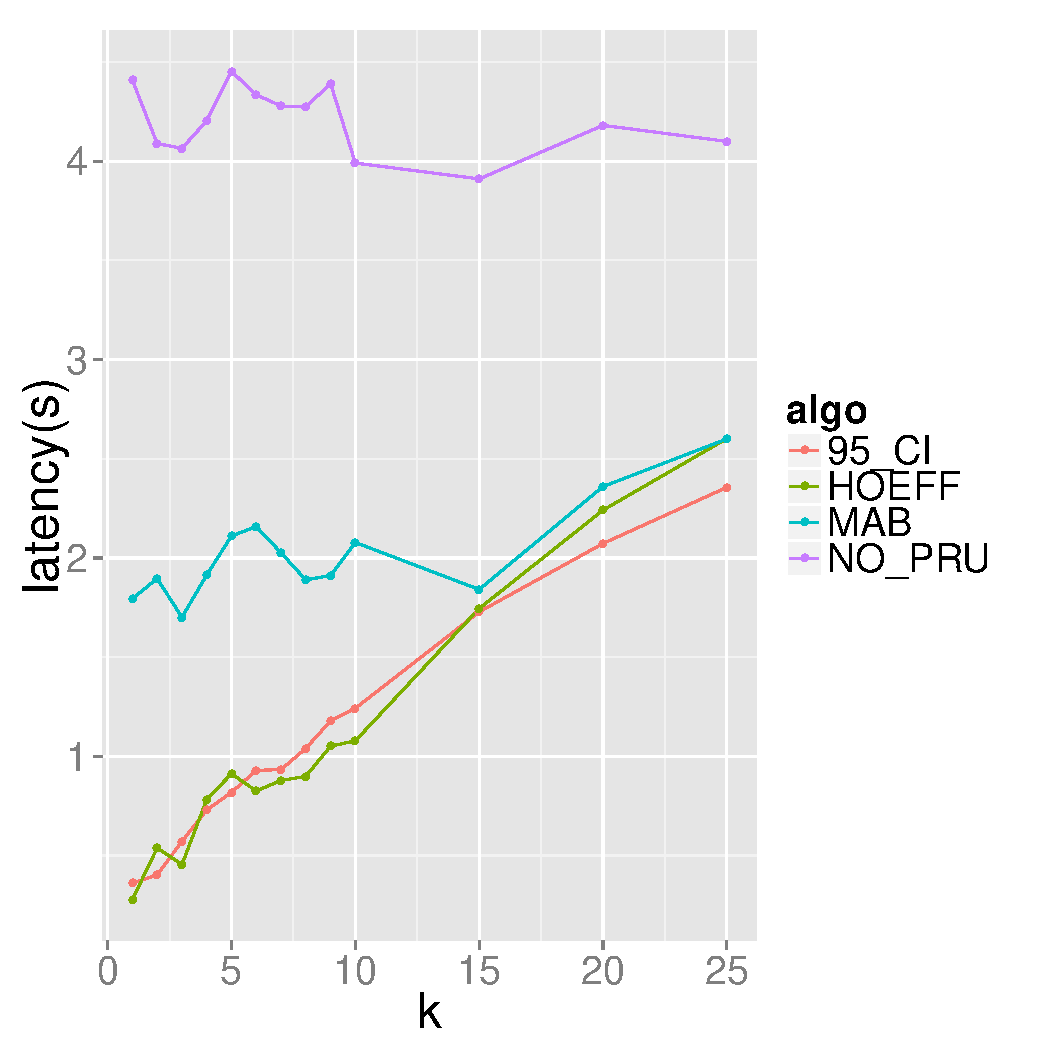
\includegraphics[width=4.2cm] {Images/bank_in_memory_latency.pdf}}
% \caption{Bank dataset: latency}
% \label{fig:bank_latency}
% \end{subfigure}
% \begin{subfigure}{0.49\linewidth}
% \centering
% {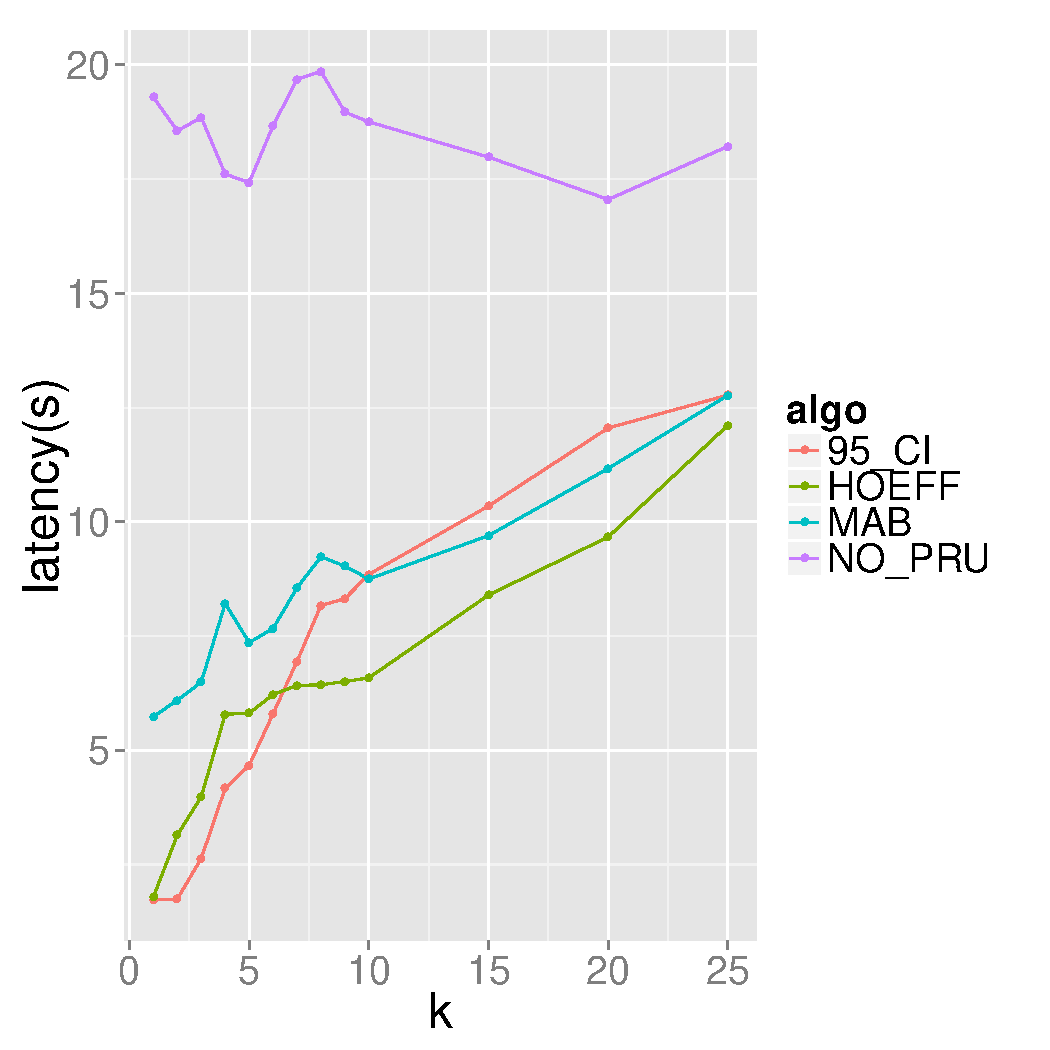
\includegraphics[width=4.2cm] {Images/dia_in_memory_latency.pdf}}
% \caption{Diabetes dataset: latency}
% \label{fig:diabetes_latency}
% \end{subfigure}
% \label{fig:accuracy}
% \caption{Latency for strategies}
% \end{figure}

% \stitle{Accuracy vs.~Latency:}
% {\em \underline{Summary:} Tuning the knobs in the pruning strategies
% gives us further reduction in latency for some losses in accuracy.}
% All of our strategies have ``knobs'' we can use to study the
% trade-off between accuracy and latency: for MAB, this corresponds to the
% number of phases used during processing while for the CI pruning, it 
% corresponds to the size of confidence intervals.
% As expected, if we set these respective parameters to favor greater accuracy 
% (i.e. fewer pruning phases in MAB or larger confidence intervals in CI pruning),
% it also leads to larger latency since fewer views can be pruned at any step.

% Here, we study the impact of these knobs on MAB and 95\_CI, which represent
% two extremes in our set of pruning strategies.
% For MAB, the knob is the number of phases involved in
% processing file; since MAB reduces the number of 
% views by 1 after each phase, the number of
% phases is proportional to the pruning power of our algorithm.
% A large number of phases means that MAB will prune more views and will prune
% them more often.
% Figure \ref{fig:latency_vs_accuracy_mab} shows how latency and accuracy both
% reduce as we increase the number of phases in MAB ($k$=15).
% Each point on the chart corresponds to a different setting for the number of
% phases uses in that implementation of the MAB strategy.
% For 95\_CI, we can vary the $z$-score used
% to determine the size of our confidence intervals.
% That is, we can decide to take a 50\% confidence interval or a 80\% interval or
% a 95\% interval.
% If we take a smaller confidence interval, we will have higher pruning and
% therefore lower latency.
% However, a smaller confidence interval also leads to lower latency since we
% prune views with lower confidence.
% Figure \ref{fig:latency_vs_accuracy_ci} shows that as the $z$-score of the
% confidence interval increases, the accuracy of our strategies increases, but so
% does its latency ($k$=15).
% Every point corresponds to a different size of the confidence intervals.

% \begin{figure}[h] 
% \centering
% \vspace{-10pt}
% \begin{subfigure}{0.49\linewidth}
% \centering
% {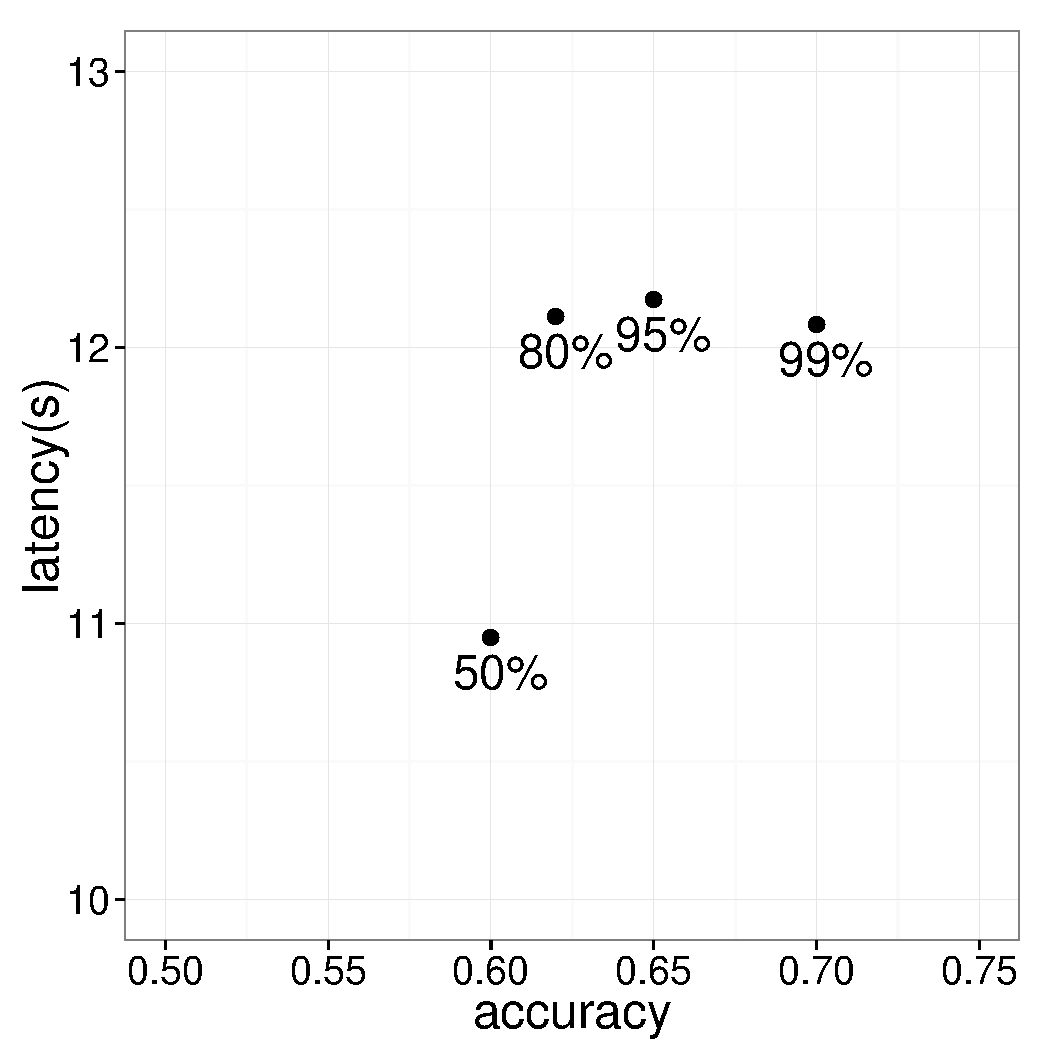
\includegraphics[width=4.2cm] {Images/latency_vs_accuracy_ci.pdf}}
% \caption{95\_CI: Values depict CI \%}
% \label{fig:latency_vs_accuracy_ci}
% \end{subfigure}
% \begin{subfigure}{0.49\linewidth}
% \centering
% {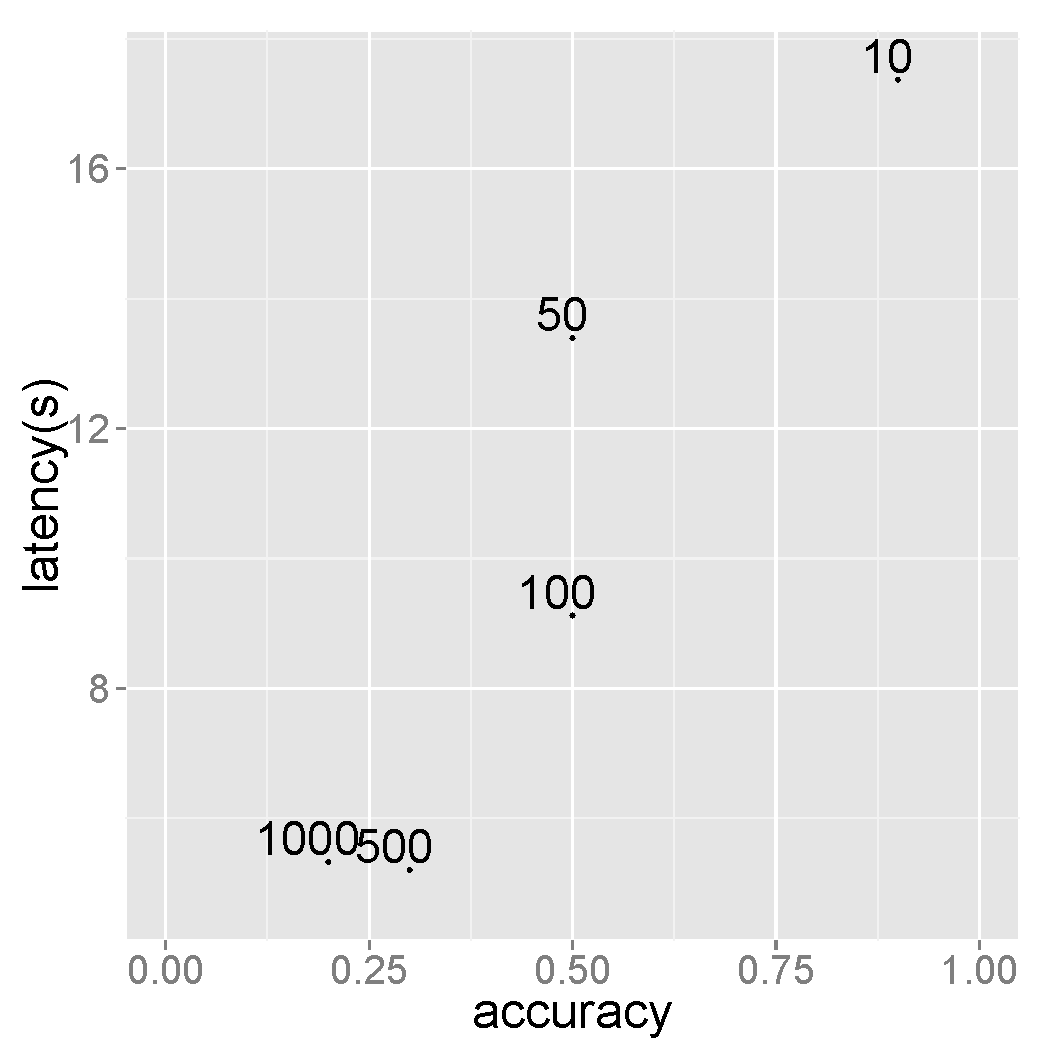
\includegraphics[width=4.2cm] {Images/latency_vs_accuracy_mab.pdf}}
% \caption{MAB: Values depict no. of phases}
% \label{fig:latency_vs_accuracy_mab}
% \end{subfigure}
% \label{fig:accuracy}
% \vspace{-10pt}
% \caption{Latency vs. Accuracy for different strategies}
% \vspace{-20pt}
% \end{figure}

